

% ---------------------------------------------------------------------------
% A3 -- backs the "stays roughly flat and recomposes" claim (src:motivation)
% with the coverage-robust composition data. Count LEVELS are contaminated by
% the 2024 SIG coverage artifact, so nothing here is a volume trend: the LHS
% is a within-cycle SHAPE (each year normalized to its own total) and the RHS
% is all shares/ratios. Numbers come from litigation_composition.tex, generated
% by 01_descriptives.py -- nothing hard-coded.
% ---------------------------------------------------------------------------
\begin{frame}{Recomposition Without Aggregate Growth}
\hypertarget{app:recomp}{}
\footnotesize
The adversarial arena rearranges rather than expands. Filings run later in the cycle, leaving a fatter post-election tail; they escalate further, with more appeals and higher per-candidate intensity; and they tilt toward gender-quota fraud, while the broad topic mix barely moves.
\smallskip
\begin{columns}[T]
\begin{column}{0.50\linewidth}
\centering
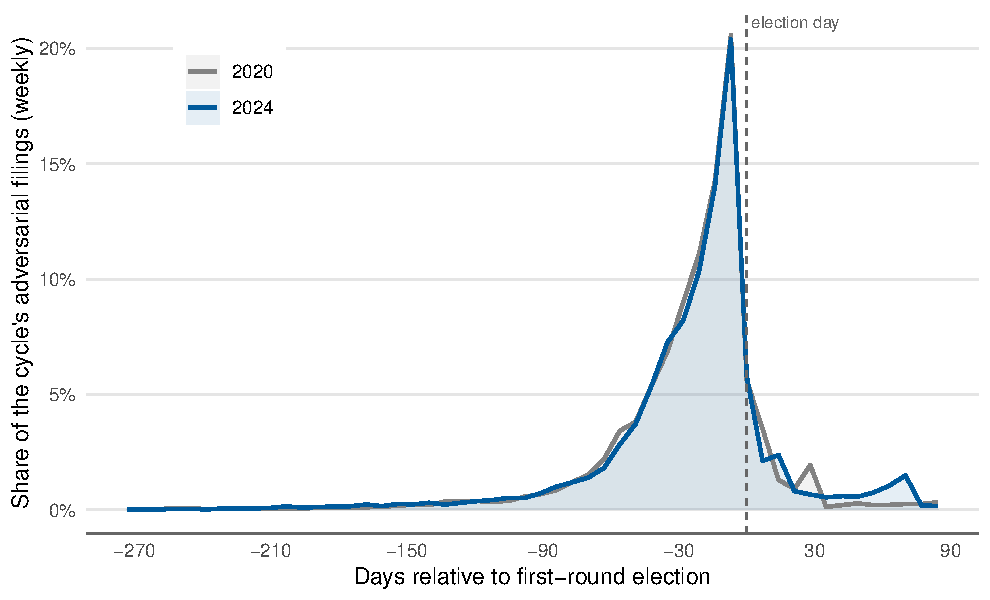
\includegraphics[width=\linewidth,height=0.44\textheight,keepaspectratio]{../figures/litigation_timing_shape.pdf}\\[4pt]
{\scriptsize\ns{Filings by week relative to the vote, each cycle normalized to its own total. Both peak in the final fortnight; 2024 (blue) carries the fatter post-vote tail.}}
\end{column}
\begin{column}{0.48\linewidth}
\centering
\resizebox{\linewidth}{!}{% Auto-generated by code/04_analysis/01_descriptives.py
% Do not edit manually -- rerun the generating script to update

\begin{tabular}{lcc}
\toprule\toprule
 & \textbf{2020} & \textbf{2024} \\
\midrule
\multicolumn{3}{l}{\textit{Within-adversarial composition (share of filings)}} \\
Campaign conduct & 0.520 & 0.516 \\
Information environment & 0.402 & 0.387 \\
Abuse / misuse of office & 0.060 & 0.074 \\
Eligibility \& ballot access & 0.018 & 0.022 \\
\midrule
\multicolumn{3}{l}{\textit{Character of the arena}} \\
Post-election filing share & 0.268 & 0.297 \\
Appeal escalation rate & 0.046 & 0.052 \\
Adversarial appeals per 1{,}000 candidates & 31.5 & 46.9 \\
\bottomrule\bottomrule
\end{tabular}
}\\[4pt]
{\scriptsize\ns{Topic shares (top) barely move, while the character rows (bottom) do: filings run later, appeal more, and per-candidate escalation rises by half.}}
\end{column}
\end{columns}
\smallskip
{\centering\scriptsize This matters for identification because the recomposition is national, and it reaches each municipality through that municipality's own 2020 topic mix. The same shift produces unequal local exposure, which is the variation the instrument uses.\par}
\smallskip
\end{frame}
